\begin{figure}[h!]

\centering

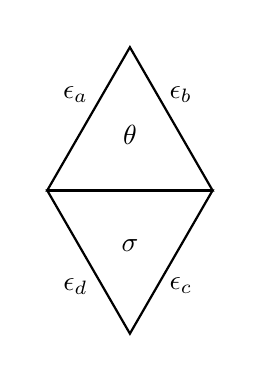
\begin{tikzpicture}[scale=0.7, baseline, thick]

\draw (0,0)--(3,0)--(60:3)--cycle;

\draw (0,0)--(3,0)--(-60:3)--cycle;

\draw (0,0)--node {\midarrow} (3,0);

\draw node[above] at (70:1.5){$\epsilon_a$};

\draw node[above] at (30:2.8){$\epsilon_b$};

\draw node[below] at (-30:2.8){$\epsilon_c$};

\draw node[below=-0.1] at (-70:1.5){$\epsilon_d$};

%\draw node[above] at (1,-0.12){$e$};

\draw node[left] at (0,0) {};

\draw node[above] at (60:3) {};

\draw node[right] at (3,0) {};

\draw node[below] at (-60:3) {};

\draw node at (1.5,1){$\theta$};

\draw node at (1.5,-1){$\sigma$};

\end{tikzpicture}
\begin{tikzpicture}[baseline]

\draw[->, thick](0,0)--(1,0);

\node[above]  at (0.5,0) {};

\end{tikzpicture}
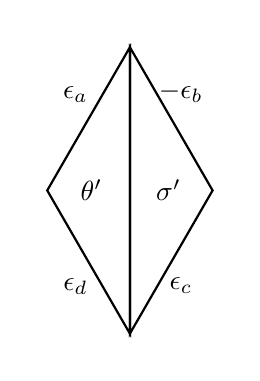
\begin{tikzpicture}[scale=0.7, baseline, thick,every node/.style={sloped,allow upside down}]
\draw (0,0)--(60:3)--(-60:3)--cycle;
\draw (3,0)--(60:3)--(-60:3)--cycle;

\draw node[above] at (70:1.5){$\epsilon_a$};

\draw node[above] at (30:2.8){$-\epsilon_b$};

\draw node[below] at (-30:2.8){$\epsilon_c$};

\draw node[below=-0.1] at (-70:1.5){$\epsilon_d$};

\draw (1.5,-2) --node {\midarrow} (1.5,2);

%\draw node[left] at (1.7,1){$f$};

\draw node[left] at (0,0) {};

\draw node[above] at (60:3) {};

\draw node[right] at (3,0) {};

\draw node[below] at (-60:3) {};

\draw node at (0.8,0){$\theta'$};

\draw node at (2.2,0){$\sigma'$};

\end{tikzpicture}
\begin{tikzpicture}[baseline]

\draw[->, thick](0,0)--(1,0);

\node[above]  at (0.5,0) {};

\end{tikzpicture}
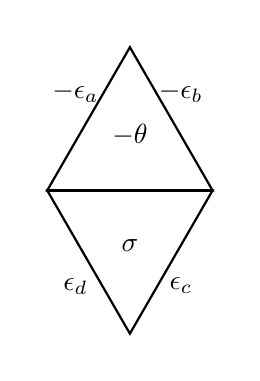
\begin{tikzpicture}[scale=0.7, baseline, thick]

\draw (0,0)--(3,0)--(60:3)--cycle;

\draw (0,0)--(3,0)--(-60:3)--cycle;

\draw (3,0) --node {\reflectbox{\midarrow}} (0,0);

\draw node[above] at (70:1.5){$-\epsilon_a$};

\draw node[above] at (30:2.8){$-\epsilon_b$};

\draw node[below] at (-30:2.8){$\epsilon_c$};

\draw node[below=-0.1] at (-70:1.5){$\epsilon_d$};

%\draw node[above] at (1,-0.12){$e$};

\draw node[left] at (0,0) {};

\draw node[above] at (60:3) {};

\draw node[right] at (3,0) {};

\draw node[below] at (-60:3) {};

\draw node at (1.5,1){$-\theta$};

\draw node at (1.5,-1){$\sigma$};

\end{tikzpicture}
\caption{Flip effect on spin structures. Here $\epsilon_x$ denotes the orientation of an edge $x$.}
\label{fig:flip_spin}
\end{figure}
